% Chapter Template

\chapter{Caso d'uso: fine-tuning su dataset arbitrario} % Main c
\label{Capitolo6} % Change X to a consecutive number; for referencing this chapter elsewhere, use \ref{ChapterX}
\def \path {Figures/C6}
Un tipico scenario d'uso industriale è quello di avere un piccolo dataset di immagini annotate a disposizione e, da questo, dover costruire un modello che riesca a generalizzare bene su esempi ancora mai visti. In questo capitolo si vedrà come affrontare questo problema utilizzando le convolutional neural networks ed il \emph{transfer learning}.


di prendere una rete allo stato dell'arte, già addestrata per mesi su per utilizzarla su un dataset arbitrario a nostra scelta, per scopi industriali o personali.
%--------------------------------------------------------------------
%	SECTION 1
%--------------------------------------------------------------------
\section{Il problema}
Occorre trovare una maniera di costruire un modello che riesca ad essere addestrato su un dataset discretamente piccolo ma al contempo sia successivamente capace di classificare correttamente esempi ancora non visti. Le CNN sono la norma quando si tratta di task di classificazione, tuttavia è difficile riuscire ad affrontare un problema del genere per i seguenti motivi: 
\begin{enumerate}
\item un modello troppo semplice non sarebbe capace di estrarre tutte le caratteristiche necessarie per catalogare le immagini; 
\item addestrare finemente un modello complesso richiede delle risorse computazionali non indifferenti, non a disposizione;
\item un modello troppo complesso con un dataset troppo piccolo avrebbe la certezza di incorrere in overfitting.
\end{enumerate}
\\
In pratica, in pochi addestrano interamente una CNN da zero proprio per i problemi elencati sopra. Quello che in genere si fa è usare modelli pre-addestrati per settimane su un dataset enorme come quello di \emph{Imagenet\href{http://www.image-net.org/}} come estrattori di features da applicare a dataset più piccoli per i più svariati scopi.


%--------------------------------------------------------------------
%	SECTION 2
%--------------------------------------------------------------------
\section{Transfer Learning & Fine-tuning}
Sfruttare l'apprendimento di grosse CNN per trasferirlo alla nostra rete è un processo che prende il nome di \emph{"transfer learning"}. \\
Gli scenari principali del transfer learning sono i seguenti: 
\begin{itemize}	
\item \textbf{CNN come estrattore di feature}: si prende una rete addestrata su ImageNet, si rimuove l'ultimo strato completamente connesso che faceva da classificatore per le 1000 classi di ImageNet, e si utilizza la restante rete come estrattore di features per il nuovo dataset. Si danno in ingresso alla rete le immagini del nuovo dataset e si ottengono in uscita le attivazione dell'ultimo hidden layer prima del classificatore finale, chiamate anche \emph{CNN codes}. Una volta ottenuti questi CNN codes, gli si addestra un classificatore lineare (una SVM o un SoftMax).
\\
Uno schema di questo approccio si è visto nella figura \ref{fig:cnn1} del Capitolo \ref{Capitolo3}, dove il primo rettangolo rossa indica la CNN come estrattore di features. 
\end{itemize}
\parencite{Wzoo}


\section{Dataset}






%--------------------------------------------------------------------
%	SECTION 3
%--------------------------------------------------------------------

\section{ModelZoo}

\subsection{Fine-tuning su Resnet}
Facebook ha reso pubbliche le sue implementazioni di Resnet su github a tutti, cosicché possano essere utilizzate per qualsivoglia esperimento. Ci sono vari modelli, più o meno potenti a seconda degli strati della rete (da 18 a 140). 

QUA INSERIRE LA FIGURA DISEGNATA SU DRAW.IO 

\begin{figure}[h!]
 \centering
 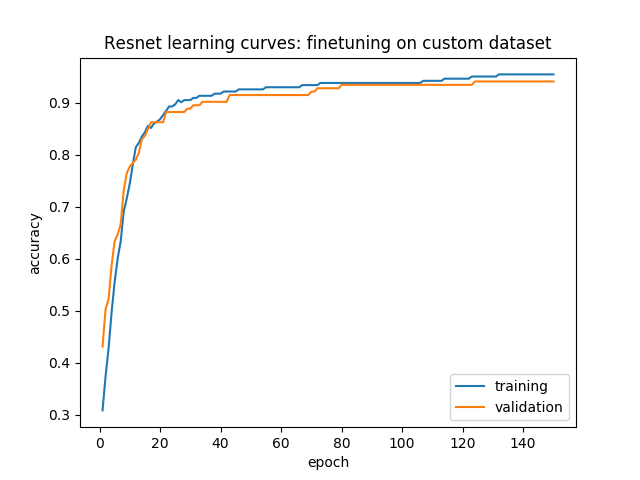
\includegraphics[width=1.0\textwidth]{\path/Figure1.png} 
 \caption{Curve di apprendimento sul nuovo dataset: il modello generalizza in maniera ottimale e non vi sono segni di overfitting}
 \label{fig:res-train}
\end{figure}

\begin{figure}[h!]
 \centering
 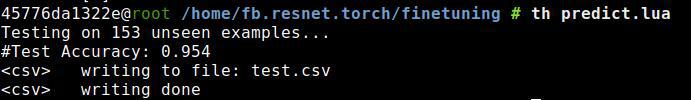
\includegraphics[width=1.0\textwidth]{\path/test-unseen-data.jpg} 
 \caption{Testing della rete su 154 esempi ancora non visti. Accuracy = 95.4\%}
 \label{fig:res-train}
\end{figure}

\begin{lstlisting}[language={[5.2]Lua}]
--add a Log-SoftMax classifier at the end of the Net
model:add(nn.LogSoftMax())

--criterion (i.e. the loss) will be the negative-likelihood
criterion = nn.ClassNLLCriterion()
\end{lstlisting}
